\section{\label{formal-model} A Formal Model for DNS}

In this section, we define a formal model for DNS and provide the semantics
for all its syntactic components, viz. authoritative nameservers and
recursive resolvers. In \Cref{subsec:trcps}, we first define the meta-model of recursive communicating processes with timers, which is a timed extension of the commonly known model of recursive communicating processes. In  Sections~\ref{subsec:dns-semantics}--\ref{subsec:RR-semantics},
we use our meta-model to comprehensively capture complex features such as recursive subqueries, time-to-live (TTL) records, channel communication, non-determinism, etc. In particular, authoritative nameservers are modelled as LTS components and the recursive resolver is modelled as a tPDS component, allowing it to use timers, for keeping track of the age of cache elements, and a stack, to simulate recursive subquery resolution. As shown in Section \ref{sec:property-agnostic}, we provide a reduction of this model to a recursive CPS.



\subsection{Definitions and Notations}\label{subsec:def-not}
Consider a monoid $\cal M = \tup{M,\cdot, \mathbf{1}}$, where $M = \tup{G}$ is generated by the subset $G \subseteq M$, with the binary operation ($\cdot$), and the identity element $\mathbf{1}$. Given any two subsets $B,C \subseteq M$, we define the sets, $B\cdot C \coloneqq \{x\cdot y\mid x\in B, y\in C\}$, and $m\cdot B \coloneqq \{m\cdot x \mid x\in B\}$, for an arbitrary $m \in M$.

\subsubsection{Domain names and IP addresses}
An IP address is a string $ip\in \scrsf{ip}$, where $\scrsf{ip}$ is the set of all IP addresses, disjoint from $M$. A \emph{domain name} over $\monoid$ is a string $d \in M$ used to point to an IP address. The identity element $\mathbf{1}$ represents the root domain name. Henceforth, as a convention, we write our domain names in the \emph{reverse order}, starting with the labels higher up in the namespace hierarchy. For example, we will write \name{com.example.www} instead of \name{www.example.com}. For better readability, the set of all domain names over $\monoid$ is denoted by $\scrsf{domain}\subsub{\monoid} = M$.





\subsubsection{Resource records}

A \emph{resource record} $rr=\tup{d,t,\sigma,v,b}$ is a tuple consisting
of a \emph{record name} $d\in\scrsf{domain}\subsub{\monoid} \cup \scrsf{domain}\subsub{\monoid_{\star}}$ where
$\scrsf{domain}\subsub{\monoid_{\star}}$ denotes the set of domain names in wildcard records over the isomorphic monoid $\monoid_{\star} = \tup{M_\star = \tup{G_\star},\ostar,\mathbf{1}_{\star}}$ where $G_\star = \{g_\star \mid g\in G\}$, such that $m_{\star}\ostar m_{\star}' = (m \cdot m')_{\star}$; the record type $t\in\scrsf{type}=\{\scrsf{a},\scrsf{ns},\scrsf{mx},\scrsf{dname},\scrsf{cname},\scrsf{soa},\ldots\}$;
a time-to-live value $\sigma\in\mathbb{N}$; the value of the record
$v\in\scrsf{ip}\cup\scrsf{domain}\subsub{\monoid}$;
and a bit value $b\in\{0,1\}$ that denotes whether the record has
been synthesized from a $\scrsf{dname},\scrsf{cname}$, or $\scrsf{wildcard}$
record. We shall write dn$(rr)$, ty$(rr)$, ttl$(rr)$, val$(rr)$, and syn$(rr)$, to denote the fields $d,t,\sigma,v$, and $b$, in $rr$,
respectively. The class of all resource records is denoted by $\scrsf{record}\subsub{\monoid}$.

A \emph{zone} is a set of resource records. The set of all zones is denoted
by $\scrsf{zone}\subsub{\monoid}={\cal P}(\scrsf{record}\subsub{\monoid})$. Additionally, we assume
all zones are \emph{well-formed}, as described in \cite[Appendix A]{groot}. We shall
write $\text{dn}(z)$ to denote the domain name of a well-formed zone.

A \emph{zone file configuration} (ZFC) is a pair, $\tup{\cal Z, \Theta}$, consisting of a function $\cal Z : \cal S \rightarrow \cal P(\scrsf{zone}\subsub{\monoid})$ from a finite set $\cal S \subseteq \scrsf{ip}$ of IPs to the powerset of $\scrsf{zone}\subsub{\monoid}$, along with a subset $\Theta \subseteq \cal S$. Intuitively, $\cal S$ denotes a set of nameservers and $\Theta$ denotes the set of root nameservers in the network; $\cal Z(s)$ denotes the set of zones for which $s$ is authoritative. The set of all ZFCs is denoted by $\scrsf{zfc}\subsub{\monoid}$.

\subsubsection{Queries}

A DNS \emph{query} $q=\tup{d,t}$ is a pair consisting of a domain
name $d\in\scrsf{domain}\subsub{\monoid}$ and the type of query $t\in\scrsf{type}$.
For example, a query expecting a $\rtype{dname}$ rewrite for the domain name
$\mathsf{{com.example}}$ would be $\tup{\mathsf{com.example},\scrsf{dname}}$.
The set of all queries is denoted by $\scrsf{query}\subsub{\monoid}=(\scrsf{domain}\subsub{\monoid}\times\scrsf{type})\uplus\{\bot\}$,
where $\bot$ denotes a non-existent query. We shall write $\text{dn}(q)$
and $\text{ty}(q)$ to denote the fields $d$ and $t$.

\subsubsection{Answers}

\sloppy Every DNS \emph{answer} $a=\tup{l,rec}$ is a pair consisting of
a label $l\in\{\scrsf{ans},\scrsf{ansq},\scrsf{ref},\scrsf{rec},\scrsf{nxdomain},\scrsf{refused}\}$
denoting the type of answer (i.e., an answer $\scrsf{ans}$, a rewrite
$\scrsf{ansq}$, a delegation $\scrsf{ref}$, a recursive subquery
request $\scrsf{rec}$, an indication for a non-existent domain name query $\scrsf{nxdomain}$, etc.) and a set of resource records $\mathit{rec}\in\mathcal{P}(\scrsf{record}\subsub{\monoid})$
that contains information for further evaluation. The set of all answers is denoted by $\scrsf{answer}\subsub{\monoid}$.

\subsubsection{Server List}

A \emph{server list} $sl \in M^*$, is a string of domain names where each domain name is unique. That is, $sl[i] \neq sl[j]$, for $0\leq i < j \leq |sl|$. The set of all server lists is denoted by $\scrsf{slist}\subsub{\monoid}$. We additionally define a left action, $\odot$, of $M$ on $\scrsf{sl}\subsub{\monoid}$ such that for any $m\in M$, 
\[m \odot sl = \begin{cases}
	(m)(sl), & \text{if } m \text{ does not match any position in } sl\\
	(m)(sl'), & \text{otherwise,}
\end{cases}\]
where $sl'$ is the string derived from $sl$ by dropping the (only) position labelled by $m$. Given a string $\mathbf{m} = m_1\ldots m_n \in M^*$, we denote by $\mathbf{m}\odot sl$, the right associative composition of actions $m_1\odot (\ldots \odot(m_n \odot sl))$.

\Cref{fig:DNS-notation} describes some notation we use
when specifying DNS behavior, along with the intended semantics. $\scrsf{rank}$ adopts the product ordering $\vartriangleleft$
over the order $\mathit{false}\leq \mathit{true}$ of truth values. 

\begin{figure}
	\begin{tcolorbox}[width=\linewidth]
        \scalebox{.75}{ 
            \parbox{\linewidth}{ 
			\begin{align*}
				d_1^{-1} \cdot d_2 & \coloneqq \{d \mid d\in M, d_1\cdot d = d_2\} & \text{\emph{domain inverse relation}}\\
				prec(d) & \coloneqq \{d_1 \mid d \in d_1 \cdot M\} & \text{\emph{domain prefix set}}\\
				d_{1}\simeq_{j}d_{2} & \coloneqq |prec(d_1) \cap prec(d_2)| \geq j - 1 & \text{\emph{domain prefix match}}\\
				max_{\simeq}(d_{1},d_{2}) & \coloneqq |prec(d_1) \cap prec(d_2)| - 1 & \text{\emph{maximal prefix match}}\\
				d_{1} < d_{2} & \coloneqq prec(d_1) \subset prec(d_2) & \text{\emph{domain partial order}}\\
				\text{dn}(rr)\ni_{{\star}} d & \coloneqq d_\star \in \text{dn}(rr)\ostar G_\star \wedge \text{dn}(rr)\in M_\star & \text{\emph{domain wildcard match}}\\
				\scrsf{wildcard}(rr) & \coloneqq \text{dn}(rr) \in M_\star & \text{\emph{wildcard record}}\\
				\scrsf{match}(rr,d) & \coloneqq \text{dn}(rr)\ni_{{\star}} d \vee (d \in \text{dn}(rr)\cdot M \wedge \text{dn}(rr)\in M) & \text{\emph{record matches query}}\\
				\scrsf{rank}(rr,\tup{d,t},z) & \coloneqq\tup{\scrsf{match}(rr,d),\text{ty}(rr)=\scrsf{ns}\wedge\text{dn}(rr)\neq\text{dn}(z),max_{\simeq}(\text{dn}(rr),d),\scrsf{Wildcard}(rr)} & \text{\emph{resource record rank}}\\
				rr_1<_{q,z}rr_2 & \coloneqq\scrsf{rank}(rr_1,q,z)\vartriangleleft\scrsf{rank}(rr_2,q,z) & \text{\emph{resource record order}}
			\end{align*}
}}   
	\end{tcolorbox}
	\captionsetup{skip=0pt}
	\caption{\label{fig:DNS-notation}Some DNS notation.} 
\end{figure}

\begin{example}\label{ex:normal-domain}
	Consider the free monoid of strings $\cal L = \tup{\scrsf{label}^*,(.),\epsilon}$, generated by an infinite set of labels $\scrsf{label}$ under concatenation. The strings $\mathsf{com.example.a}$ and $\mathsf{com.example.b}$ are examples of domains in $\scrsf{domain}_{\cal L}$, if the labels $\mathsf{com,example,a,b}\in \scrsf{label}$. The empty string $\epsilon$ represents the root domain. 
	
	The expression $(\mathsf{com}^{-1}.\mathsf{com.example.a})$ denotes the singleton set $\{\mathsf{example.a}\}$; $prec(\mathsf{com.example.a})$ is the set of prefixes $\{\epsilon, \mathsf{com,com.example,com.example.a}\}$; $max_{\simeq}(\mathsf{com.example.a},\mathsf{com.example.b})$ is $2$, the size of the set $\{\mathsf{com,com.example}\}$, of non-trivial common prefixes; consequently, $(\mathsf{com.example.a}\simeq_{1}\mathsf{com.example.b})$ holds; however, $(\mathsf{com.example.a}\leq\mathsf{com.example.b})$ does not hold as $\mathsf{com.example.a}\not\in prec(\mathsf{com.example.b})$.
\end{example}

The next lemma follows immediately from our definitions.

\begin{lemma}\label{lem:notation-functorial}
	The sets $\scrsf{domain}\subsub{\monoid},\scrsf{record}\subsub{\monoid},\scrsf{zone}\subsub{\monoid}, \scrsf{zfc}\subsub{\monoid}, \scrsf{query}\subsub{\monoid}$, $\scrsf{answer}\subsub{\monoid}$, and $\scrsf{slist}\subsub{\monoid}$ are all functorial\footnote{Given an expression $A$ that contains $B$, we say that $A$ is \emph{functorial} in $B$, if $B \mapsto A$ is a functor.} in the monoid $\monoid$.
\end{lemma}

Notably, IP addresses remain unchanged with the change in the underlying monoid $\monoid$.

\subsection{Recursive Communicating Processes with Timers\label{subsec:trcps}}
We will now introduce the notion of recursive communicating processes with timers, extending the model of recursive communicating processes (rCPS) \cite{heussner2010reachability,heussner2012reachability}, where finitely many processes communicate with each other over perfect channels, dictated by an underlying topology. Therefore, we first define the notion of a network topology, which is a directed graph whose vertices represent processes and whose edges represent channels.
\begin{definition}
	A \emph{network topology} $\cal T$ is a 3-tuple $\tup{P,\scrsf{ch},\ch}$, where $P$ is a finite set of processes, $\scrsf{ch}$ is a finite set of perfect channel identifiers, and $\ch : \scrsf{ch} \rightharpoonup P \times P$ is a partial map from channel identifiers to the processes it connects.
	
	We write $\ch_{c}$ to denote the channel from the \emph{source} process $i \in P$ to the \emph{destination} process $j \in P$, if $\ch(c) = \tup{i,j}$. Moreover, we assume that $\ch^{-1}(\tup{i,i})$ is always empty i.e., there is no channel from a process to itself.
\end{definition}

Consider a network topology $\mathsf T = \tup{P,\scrsf{ch},\ch}$. Given a message alphabet $M$, we define the set of \emph{channel actions}, $\scrsf{caction}_{\mathsf T,M}^p = \{\ch_c!a \mid c \in \ch^{-1}\tup{p,p'}, p'\in P, a \in M\} \cup \{\ch_c?a \mid c \in \ch^{-1}\tup{p',p}, p'\in P, a \in M\}$ for every $p \in P$. The operations of the form $\ch_c?a$ and $\ch_{c}!a$ denote the actions of \emph{receiving} and \emph{sending} the message $a$ on channel $\ch_c$ respectively. 

Next, we define the model of pushdown systems with timers and a timeless stack, where we follow the model proposed in \cite[\S 2]{clemente2015timed}, but use timers \cite{vaandrager2023learning,KuroseRoss16} instead of clocks.\footnote{The restriction to timers reduces the space complexity of the abstract configuration space we introduce in Section~\ref{subsec:abstract-model}. From a decidability perspective, all the reductions presented in this paper hold for the more expressive class of timed pushdown systems proposed in \cite{clemente2015timed}.} Unlike clocks, timers run \emph{backwards}, starting from an initial value. Moreover, we restrict the timing constraints to \new{only allow \emph{timeout checks}}. A \emph{timing constraint} over a set of timers $X$ is a formula generated by the grammar,
\[ \scrsf{cc}\subsub{X} \coloneqq x > 0 \mid \scrsf{cc}\subsub{X} \wedge \scrsf{cc}\subsub{X},\]
where $x\in X$ and timer resets are represented by $[\mathbf{x} \leftarrow \mathbf{k}]$, with $\mathbf{k} \in \mathbb{N}^n$; $\mathbf{x}\in X^n$ is a vector with distinct timer components, denoting that each timer $\mathbf{x}_i$ in $\mathbf{x}$ is reset to the value $\mathbf{k}_i$.

A \emph{timer valuation} over $X$ is a map $\nu : X \rightarrow \rat^{\geq 0} \cup \{\infty\}$, where $X$ is a set of timers and each timer either holds a non-negative rational number (denoted by $\rat^{\geq 0}$) or it has not yet been initialized (denoted by $\infty$). Given $k \in \rat^{\geq 0}$, we denote by $\nu - k$ the valuation, where for each $x\in X$, 
\[(\nu - k)(x) = \begin{cases}
	\nu(x) - k, & \text{if } \nu(x) \geq k\\
	0, & \nu(x) < k\\
	\infty, & \nu(x) = \infty.
\end{cases}\]
Given a vector $k \in \nat^n$, we denote by $\nu[\mathbf{x} \leftarrow \mathbf{k}]$ the updated timer valuation such that $\nu[\mathbf{x} \leftarrow \mathbf{k}](x) = k_i$ if $x = \mathbf{x}_i$ for some $i$; otherwise, $\nu[\mathbf{x} \leftarrow \mathbf{k}](x) = \nu(x)$.\footnote{Note that the semantics of a timer is less expressive than that of a clock. However, since most implementations of $\scrsf{dns}$ use the notion of timer-based timeouts in their states, using timers greatly simplifies further reductions in this paper.}

\begin{definition}\label{def:tpds}
	A \emph{pushdown system with timers} (tPDS) is a 6- tuple $\cal P = \tup{S,S_{init},A,\Gamma,X,\trans}$, where $S$ is a finite set of states, $S_{init} \subseteq S$ is a finite set of initial states, $A$ is a finite input alphabet, $\Gamma$ is a finite stack alphabet, $X$ is a finite set of timers, and $\trans$ is a set of transition rules. The transition rules are of the form $s \xrightarrow[{[\mathbf{x} \leftarrow \mathbf{k}]},cc]{\tup{\alpha,a,\alpha'}} s'$, with $s,s' \in S$ states, $a \in A \cup \{\epsilon\}$ an input letter, and $\mathbf{x} \in X^n$ an n-dimensional vector of timers, being reset to $\mathbf{k}$, for some $n$; $cc \in \scrsf{cc}_X$ is a timer constraint; $\alpha\in \Gamma^*$ represents the finite lookup of the top of the stack, and $\alpha'\in \Gamma\cup \varepsilon$ represents the element to be pushed (or none thereof, if $\alpha' = \varepsilon$). The \emph{size} of $\cal P$ is the cumulative size of all its components.
\end{definition}

A \emph{configuration} $C$ of the tPDS is a 3-tuple $\tup{s,\nu,\gamma}$, where $s\in S$, $\nu$ is a \emph{timer valuation} over $X$, and $\gamma \in \Gamma^*\bottom$ is the stack valuation with the stack top being the leftmost label in $\gamma$, and the special symbol $\dashv\,\notin \Gamma$ denoting the bottom of the stack. The set of all configurations is the set $\config{\cal P} = S\times (\rat^{\geq 0} \cup \{\infty\})^X \times \Gamma^*\bottom$. The set of initial configurations is $\config{\cal P}_{init} = S_{init}\times \{\infty\}^{X} \times\{\dashv\}$. A configuration in $\{s\} \times (\rat^{\geq 0} \cup \{\infty\})^Xg \times \Gamma^*\bottom$, for $s \in S$, is called an $s$\emph{-configuration}.

The semantics for the tPDS is the LTS $\tup{\cal P} = \tup{\config{\cal P},\config{\cal P}_{init},A',\trans'}$, where $A' = ((\Gamma^*\cup\Gamma^+\bottom) \times A \times (\Gamma \uplus \{\varepsilon\})) \times \{[\mathbf{x} \leftarrow \mathbf{k}] \mid \mathbf{x} \in X^n, \mathbf{k} \in \nat^n, n \in \nat \} \times \scrsf{cc}_X$ and $\trans'$ contains two kinds of transitions:
\begin{enumerate}[(i)]
	\item \emph{timed transitions} labelled by $t \in \rat^{\geq 0}$, such that $\tup{s, \nu, \gamma} \xrightarrow{t} \tup{s, \nu - t, \gamma}$, and
	\item \emph{discrete transitions}, such that $\tup{s, \nu, \gamma} \xrightarrow[{[\mathbf{x} \leftarrow \mathbf{k}]},cc]{\tup{\alpha,a,\alpha'}} \tup{s',\nu',\gamma'}\in \trans'$, whenever $\nu \models cc$, $\nu' = \nu[\mathbf{x} \leftarrow \mathbf{k}]$, $s \xrightarrow[{[\mathbf{x} \leftarrow \mathbf{k}]},cc]{\tup{\alpha,a,\alpha'}} s' \in \trans$, and we have, 
	\[\gamma' = \begin{cases}
		\alpha'\gamma, & \text{if } \alpha' \neq \varepsilon,\alpha = \epsilon\\
		\gamma, & \text{if } \alpha' = \varepsilon,\alpha = \epsilon\\
		\gamma[1\ldots|\gamma|], & \text{if } \alpha' = \varepsilon,\alpha \neq \epsilon \text{, and } \gamma = \alpha\gamma'' \text{, for some } \gamma'\in \Gamma^*\bottom\\
		\alpha'\cdot\gamma[1\ldots|\gamma|], & \text{if } \alpha' \neq \varepsilon,\alpha \neq \epsilon \text{, and } \gamma = \alpha\gamma'' \text{, for some } \gamma'\in \Gamma^*\bottom
	\end{cases}\]
	Intuitively, each stack operation checks whether a finite length of the top of the stack matches $\alpha$, and performs either a push operation, \emph{nop} (i.e., let the stack remain the same), pop operation, or a \emph{pop and push} operation. 
\end{enumerate}
The runs of $\tup{\cal P}$ are slightly different from the definition for LTS given in \Cref{subsec:lts}. A \emph{run} in $\tup{\cal P}$ is a finite \emph{alternating} sequence of the form $\rho = C_0 \xrightarrow[{[\mathbf{x}_1 \leftarrow \mathbf{k}_1]}, cc_1]{\tup{\alpha_1,a_1,\alpha'_1}} C_1 \xrightarrow{t_1} C_1' \xrightarrow[{[\mathbf{x}_2 \leftarrow \mathbf{k}_2]}, cc_2]{\tup{\alpha_2,a_2,\alpha'_2}} C_2 \ldots C_{n-1}' \xrightarrow[{[\mathbf{x}_n \leftarrow \mathbf{k}_n]}, cc_n]{\tup{\alpha_n,a_n,\alpha'_n}} C_n$, where $t_j \in \rat^{\geq 0}$ and for every $1 \leq i \leq n$, $C_{i-1}' \xrightarrow[{[\mathbf{x}_n \leftarrow \mathbf{k}_n]}, cc_i]{\tup{\alpha_i,a_i,\alpha'_i}} C_i \in \scrsf{trans}'$. The trace of $\rho$ is the sequence $a_1\ldots a_n \in A^*$. If the set of timers $X$ is empty, $\cal P$ behaves as a standard \emph{untimed} pushdown system (PDS).

\subsubsection{Recursive Communicating Processes with Timers}
We follow the definition of an rCPS proposed in \cite[Definition 1.7]{heussner2012reachability}, extending it with timers.

A \emph{system of recursive communicating processes with timers} (trCPS) $\cal R = \tup{\mathsf T,\mathsf M, (\cal P^p)_{p \in P}}$, is given by a network topology $\mathsf T = \tup{P, \scrsf{ch}, \ch}$, a \emph{message} alphabet $\mathsf M$, and for each process $p \in P$, a tPDS $\cal P^p = \tup{S^p,S_{init}^p,A^p,\Gamma^p,X^p,\trans^p}$ such that $\scrsf{caction}^p_{\cal T, M} \subseteq A^p$. We write $\scrsf{s} = \prod_{p \in P} S^p$ for the set of \emph{global states}. The topology $\mathsf T$ is \emph{pointed} with respect to $\cal R$ if exactly one process in $P$ corresponds to a tPDS and all the others correspond to an LTS with finitely many states (see \Cref{fig:pointed-topo}).

\begin{wrapfigure}{r}{0.35\textwidth}
	\centering
  \resizebox{.24\textwidth}{!}{
	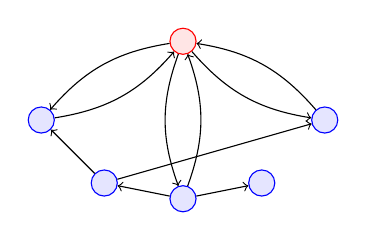
\begin{tikzpicture}%
		\node (r) [fill=red!10,draw=red,circle] at (0,0) {};
		\node (p1) [fill=blue!10,draw=blue, circle] at (0,-2) {};
		\node (p2) [fill=blue!10,draw=blue, circle] at (-1.8,-1) {};
		\node (p3) [fill=blue!10,draw=blue, circle] at (-1,-1.8) {};
		\node (p4) [fill=blue!10,draw=blue, circle] at (1.8,-1) {};
		\node (p5) [fill=blue!10,draw=blue, circle] at (1,-1.8) {};
		
		\path[->] (r) edge [bend right=20]             node              {} (p1)
		edge [bend right=20]             node              {} (p2)
		edge [bend right=20]             node              {} (p4)
		(p1) edge [bend right=20]             node              {} (r)
		edge             node              {} (p3)
		edge             node              {} (p5)
		(p2) edge [bend right=20]             node              {} (r)
		(p3) edge node {} (p2)
		edge node {} (p4)
		(p4) edge [bend right=20]             node              {} (r);
	\end{tikzpicture}
 }
	\captionsetup{skip=5pt}
	\caption{\label{fig:pointed-topo}A pointed topology. The red  process is the only tPDS in the network.}
\end{wrapfigure}

\sloppy The semantics of trCPS is defined in terms of a global LTS $\tup{\cal R} = \tup{\scrsf{config}, \scrsf{config}_{init}, \mathsf{A}, \trans}$, where $\scrsf{config} = (\config{\cal P^p})_{p \in P} \times (\mathsf M^*)^{\scrsf{ch}}$ is the set of \emph{global configurations}, $\scrsf{config}_{init} = (\config{\cal P^p}_{init})_{p \in P} \times \{\epsilon\}^{\scrsf{ch}}$ is the set of initial configurations, and $\mathsf{A} = \biguplus_{p \in P} {A'^p}$ is the set of actions. Given a \emph{global configuration} $\scrsf{c} \in \scrsf{config}$, we write $\scrsf{c}^p \in \config{\cal P^p}$ to denote the \emph{local configuration} in $\scrsf{c}$ that corresponds to the process $p \in P$, and $\scrsf{c}^{c}$ to denote the contents of channel $\ch_c$ such that $\scrsf{c}^c = \scrsf{c}^{c'}$ if $\ch_c = \ch_{c'}$. A configuration in $\scrsf{c}$ is called an $\mathbf{s}$\emph{-configuration} when, for every $p \in P$, $\scrsf{c}^p$ is an $s^p$-configuration, for some $\mathbf{s} =\tup{s^p}_{p\in P} \in \scrsf{s}$.

The discrete transitions in $\trans$ of the form $\scrsf{c} \xrightarrow[{[\mathbf{x} \leftarrow \mathbf{k}]}, cc]{\tup{\alpha,a,\alpha'}} \scrsf{c}'$, for $a\in A^p$, satisfy the following:
\begin{enumerate}[(i)]
	\item $\scrsf{c}^p \xrightarrow[{[\mathbf{x} \leftarrow \mathbf{k}]}, cc]{\tup{\alpha,a,\alpha'}} \scrsf{c}'^p \in \trans'^p$ and $\scrsf{c}^q = \scrsf{c}'^q$ for all $q\in P \setminus p$,
	\item if $a \in A^p\setminus\scrsf{caction}^p_{\cal T, M}$, $\scrsf{c}^c = \scrsf{c}'^c$ for $c \in \scrsf{ch}$,
	\item if $a = \ch_c!m$ then $\scrsf{c}'^{c''} = \scrsf{c}^{c''}\cdot m$ for each $c'' \in \ch^{-1}(\ch_c)$ and $\scrsf{c}'^{c''} = \scrsf{c}^{c''}$ for $c'' \in \scrsf{ch}\setminus\ch^{-1}(\ch_c)$,
	\item if $a = \ch_c?m$ then $m\cdot\scrsf{c}'^{c''} = \scrsf{c}^{c''}$ for each $c'' \in \ch^{-1}(\ch_c)$ and $\scrsf{c}'^{c''} = \scrsf{c}^{c''}$ for $c'' \in \scrsf{ch}\setminus\ch^{-1}(\ch_c)$.
\end{enumerate}
The timed transitions in $\trans'$ of the form $\scrsf{c} \xrightarrow{t} \scrsf{c'}$ satisfy $\scrsf{c}^p \xrightarrow{t} \scrsf{c}'^p \in {\trans^p}'$ for all $p \in P$. We will refer to runs in $\tup{\cal R}$ as runs in $\cal R$.


Observe that, if none of the component processes in a trCPS uses timing operations, our model essentially becomes a rCPS \cite[Def. 1.7]{heussner2012reachability}. Similarly, without timing and stack operations, the model becomes a CPS \cite[Def. 1.2]{heussner2012reachability}. 

\subsubsection{Eager Runs}\label{subsubsec:eagerness}
The notion of eager runs was first introduced by Heussner et. al. \cite{heussner2010reachability,heussner2012reachability}, in the context of rCPS. We will extend this notion to trCPS.

\begin{definition}
	A run $\rho = \scrsf{c}_0 \xrightarrow[{[\mathbf{x}_1 \leftarrow \mathbf{k}_1]}, cc_1]{\tup{\alpha_1,a_1,\alpha'_1}} \scrsf{c}_1 \xrightarrow{t_1} \scrsf{c}_1' \xrightarrow[{[\mathbf{x}_2 \leftarrow \mathbf{k}_2]}, cc_2]{\tup{\alpha_2,a_2,\alpha'_2}} \scrsf{c}_2 \ldots \scrsf{c}_{n-1}' \xrightarrow[{[\mathbf{x}_n \leftarrow \mathbf{k}_n]}, cc_n]{\tup{\alpha_n,a_n,\alpha'_n}} \scrsf{c}_n$ in a trCPS is \emph{eager} if for all $1 \leq i \leq n$, if $a_i$ is of the form $\ch_c?m$ then $i > 1$ and $a_{i - 1}$ is the corresponding write action $\ch_c!m$ in $\rho$. 
\end{definition}




Intuitively, \emph{eagerness} formalizes that, in a run, send actions are immediately proceeded by their matching receive actions. A configuration $\scrsf{c} \in \scrsf{config}$ is \emph{eager-reachable} in a trCPS $\cal R$ if there exists an eager run from an initial configuration in $\scrsf{config}_{\mathit{init}}$ to $\scrsf{c}$. We say that a trCPS $\cal R$ is \emph{eager} when every run in $\cal R$ is eager.
The \emph{state eager-reachability problem} for $\cal R$ asks whether, for a given global state $\mathbf{s} \in \scrsf{s}$, there exists an eager run from an initial configuration to an $\mathbf{s}$-configuration.

Heussner et. al. \cite[Prop. 2.4]{heussner2010reachability} characterized a subclass of topologies for which the state eager-reachability problem for rCPS, satisfying certain additional restrictions on their communication behaviour, is decidable. As it happens, the class of rCPS over pointed topologies satisfies these conditions; in particular, this fact is subsumed by the case $(ii)$ in their proof, where they reduce the search for an eager run in the rCPS to the search for a run in a (untimed) pushdown system. The reduced pushdown system even preserves the set of traces of all eager runs in the original rCPS. In the case of pointed topologies, such a reduction leads to a pushdown system of size polynomial in the size of each of the processes.

\begin{lemma}\label{lem:rcps-to-pds}
	Given any rCPS $\cal R$, over a pointed topology, it is $\mathsf{PolyTime}$-reducible to an untimed pushdown system $\cal P$ with the set of states as the set of global states in $\cal R$, such that, for every eager run in $\cal R$, from an $\mathbf{s}$-configuration to an $\mathbf{s}'$-configuration, there exists a run in $\cal P$, from an $\mathbf{s}$-configuration to an $\mathbf{s}'$-configuration, with the same trace.
\end{lemma}

\subsection{DNS Semantics}\label{subsec:dns-semantics}

Given an arbitrary zone file configuration $\tup{\cal Z ,\Theta} \in \scrsf{zfc}\subsub{\monoid}$, we model the corresponding instance of DNS as the trCPS $\scrsf{dns}\subsub{\cal Z}=\tup{\mathsf T\subsub{\cal Z},\mathsf M\subsub{\cal Z}, (\cal P^p)_{p\in P\subsub{\cal Z}}}$, where $\mathsf T\subsub{\cal Z} = \tup{P\subsub{\cal Z}, \scrsf{ch}\subsub{\cal Z}, \ch\subsub{\cal Z}}$, and $\mathsf M\subsub{\cal Z} = \scrsf{query}\subsub{\monoid}\uplus\scrsf{answer}\subsub{\monoid}$ is the disjoint union of the set of all queries and answers, such that the following hold:
\begin{enumerate}[(i)]
	\item $P\subsub{\cal Z} = \{ r \} \uplus \cal S \subseteq \scrsf{ip}$,
	\item $\scrsf{ch}\subsub{\cal Z} = \cal S \times \cal S \uplus \{ r \} \times \cal S \uplus \cal S \times \{ r \}$,
	\item $\ch\subsub{\cal Z}$ is the identity map,
	\item $\cal P^p$ is a tPDS of the form $\rec{p}$, if $p = r$, and an LTS of the form $\ns{p}$, otherwise.
\end{enumerate}

Intuitively, $\rec{r}$ denotes the resolver, identified by its IP address; there are no communication channels between the resolver to itself. This follows, by convention \cite{groot,dnsmaude}, from a strict restriction on our model, where we typically do not allow a nameserver to also serve as a resolver in the network. However, note that this is a logical separation, as in reality this is not the case; resolvers may indeed themselves behave as nameservers \cite{rfc1034,rfc1035} in a network; $\ns{p}$ is the formal model of a nameserver. We define these models below, in Sections \ref{subsec:NS-semantics} and \ref{subsec:RR-semantics}. Note that $\mathsf T_{\cal Z}$ is a pointed topology with only one tPDS process $\cal P^r$. \new{We shall crucially use this fact in~\Cref{sec:property-validation-to-reachability} to obtain the decidability of the $\scrsf{dnsverif}$ problem.}

Unless otherwise stated, we will implicitly assume that the underlying monoid $\monoid$ is the free monoid $\cal L$, as described in Example \ref{ex:normal-domain}. For notational convenience, we shall thus drop the corresponding subscript $\cal L$ from all our terms.  
For the rest of the paper, we also arbitrarily fix an instance of DNS with the zone file configuration $\tup{\cal Z : \cal S \rightarrow \cal P(\scrsf{zone}),\Theta}$, denoting it as $\scrsf{dns}$, by dropping the subscript $\cal Z$. If clear from the context, we shall also use $\cal Z$ interchangeably to denote both, the set of all zones in the image of the configuration, and the set of all records in those zones.

\subsection{\label{subsec:NS-semantics}Authoritative Nameserver}

An \emph{authoritative nameserver}, $\ns{s}$, identified by its IP address, $s \in \cal S$, is an LTS of the form $\tup{\scrsf{nsconfig}_s,\{\tup{\mathit{init},\bot,\bot}\},\scrsf{saction}_s,\trans_s}$, where $\scrsf{nsconfig}_s$ is the set of tuples $\{\mathit{init},\mathit{lookup},\mathit{exact},\mathit{wildcard}\}\times \scrsf{query} \times \cal R$, $\scrsf{saction}_s = \scrsf{caction}^s_{\mathsf T,M} \cup \{in\}$ with the special action label $in$ for internal actions, and $\trans_s \subseteq \scrsf{nsconfig}_s \times \scrsf{saction} \times \scrsf{nsconfig}_s$. 

Given a configuration $p = \tup{\mathit{status}, q, r}$,
\begin{enumerate}
	\item \emph{status} is $\mathit{init}$ when the nameserver does not have pending query requests, $\mathit{lookup}$ when it must start the lookup process for $q$, $\mathit{exact}$ when $\text{dn}(q)$ finds an exact match with the domain name field of some resource record in a zone that $\ns{s}$ is authoritative for, and $\mathit{wildcard}$ when $\text{dn}(q)$ finds a wildcard match with the domain name field of some resource record in such a zone.
	\item $q$ is the current query.
	\item $r$ is the identity of the resolver that the nameserver communicates with.
\end{enumerate}
\begin{figure}
	\resizebox{.75\textwidth}{!}{\begin{tcolorbox}[width=.9\textwidth]
			\begin{minipage}{\textwidth}
			\begin{align*}
		\mathcal{N}(s,q) & =max_{\text{dn}}\{z\in\mathcal{Z}(s)\mid\text{dn}(z)\leq\text{dn}(q)\} \quad
		\mathcal{M}(s,q)  =\bigcup_{z\in\mathcal{N}(s,q)}\{rr\in max_{<_{q,z}}z\}\\
		{\cal T}(s,q) & =\{rr\in{\cal M}(s,q)\mid\text{ty}(rr)=\text{ty}(q)\}\quad\quad\quad
		\tau(s,q)  =\{\text{ty}(rr)\mid rr\in{\cal M}(s,q)\}\\
		{\cal T}_{t}(s,q) & =\{rr\in{\cal M}(s,q)\mid\text{ty}(rr)=t\}\quad\quad\quad\quad\quad
		{\cal G}(s,q)  ={\cal T}_{\scrsf{ns}}(s,q)\cup{\cal G}_{A}(s,q)\\ \\
		{\cal G}_{A}(s,q) & =\{rr\in\bigcup{\cal Z}(s)\mid\exists rr'\in{\cal T}_{\scrsf{ns}}(s,q).\text{val}(rr')=\text{dn}(rr) \wedge\text{ty}(rr)=\scrsf{A}\}
	\end{align*}
	\end{minipage}
	\end{tcolorbox}}
	\captionsetup{skip=5pt}
	\caption{\label{fig:aux-op}Some auxiliary operations. }
\end{figure}


Additionally, we define auxiliary operations in Figure \ref{fig:aux-op}. They
all take the server identity $s$ and an input query
$q$ as input. ${\cal N}(s,q)$ obtains the zones whose domain names have
a maximal match with $q$. ${\cal M}(s,q)$ accumulates the resource
records with maximal $\scrsf{rank}$ in the zones in ${\cal N}(s,q)$. ${\cal T}_{t}(s,q)$ gathers the resource records in ${\cal M}(s,q)$
of type $t$. ${\cal T}(s,q)$ is a special case of ${\cal T}_{t}(s,q)$
when $t=\text{ty}(q)$. $\tau(s,q)$ gathers the types of the
resource records in ${\cal M}(s,q)$. ${\cal G}(s,q)$ yields
the $\scrsf{NS}$ records in ${\cal M}(s,q)$ that have an associated $\scrsf{A}$ record. Finally, ${\cal G}_{A}(s,q)$ denotes the set of associated $\scrsf{A}$ records. Since the operators are parameterized only by a DNS query and the
choice of nameserver, they can be computed from the current state
information in $\mathsf{NS}_{s}$.

\subsubsection{Transitions}


The transitions model the local steps taken by the nameserver during query resolution. In \Cref{fig:ns-transitions}, we illustrate a transition in this set.

\begin{figure*}[h!]
	\centering
	\resizebox{\textwidth}{!}{\begin{tikzpicture}[every label/.style={circle,draw,minimum size=9pt,inner sep=0.5pt,font=\footnotesize}]
			\node [fill=blue!10,draw,rounded corners=5pt] {$\dfrac{\text{dn}({\cal M}(s,q))<\text{dn}(q),\scrsf{dname}\in\tau(s,q), dn\in\scrsf{domain}, {\cal T}_{\scrsf{dname}}(s,q)=\{rr\}, rr'=\tup{\text{dn}(q),\scrsf{cname},\text{ttl}(rr),\text{val}(rr)\text{dn}(rr)^{-1} \text{dn}(q),1}}{\tup{\mathit{lookup},q,r}\xrightarrow{c_{(dn,s),r}!\tup{\scrsf{ansq},\{rr,rr'\}}}\tup{\mathit{init},\bot,\bot}}$};
	\end{tikzpicture}}
	\captionsetup{skip=5pt}
	\caption{\label{fig:ns-transitions}A transition in $\ns{s}$. The premise of the transition specifies the condition when the transition is taken. The action label is above the arrow.}
\end{figure*}

In this transition, the nameserver $\ns{s}$ is about to start the lookup process, initiated by the status $\mathit{lookup}$, for the current query $q$, requested by the resolver $r$. The premise component $\text{dn} (\cal M (s, q)) < \text{dn} (q)$ states that $\text{dn} (q)$ is an extension of the domain name of every resource record in $\cal M (s, q)$, where $\cal M (s, q)$ represents the set of the resource records that the nameserver may potentially send back in the response to the query $q$; the components $\scrsf{dname}\in \tau (s, q)$ and ${\cal T}_{\scrsf{dname}} (s, q) = {rr}$ state that the record $rr$ in $\cal M (s, q)$ is a $\scrsf{dname}$ record. In its response, the nameserver must send back the record $rr$ and its $\scrsf{cname}$ derivative synthesized for $q$ in order to prompt a rewrite of the query. The premise component $rr'=\tup{\text{dn}(q),\scrsf{cname},\text{ttl}(rr),\text{val}(rr)\text{dn}(rr)^{-1} \text{dn}(q),1}$ represents the synthesized record as denoted by the fact that $\text{syn} (rr') = 1$, and $\text{val}(rr')$ is the rewritten domain name. With this, the nameserver then sends the answer $\tup{\scrsf{ansq},\{rr,rr'\}}$, which prompts a rewrite ($\scrsf{ansq}$) using the records $rr$ and $rr'$, and moves back to its initial configuration. 


\begin{wrapfigure}{r}{0.3\textwidth}
	\centering
 \resizebox{.3\textwidth}{!}{
	\begin{tikzpicture}[scale=0.5,every label/.style={circle,draw,minimum size=9pt,inner sep=0.5pt,font=\footnotesize}]
		\node (r1) [fill=blue!10,draw,rounded corners=5pt] {$\dfrac{\text{dn}(\cal M (s,q))=\text{dn}(q)}{\tup{\mathit{lookup},q,r}\xrightarrow{}\tup{\mathit{exact},q,r}}$};
		\node [below=20pt,fill=blue!10,draw,rounded corners=5pt] {$\dfrac{\text{dn}(\cal M (s,q))\ni_\star\text{dn}(q)}{\tup{\mathit{lookup},q,r}\xrightarrow{}\tup{\mathit{wildcard},q,r}}$};
	\end{tikzpicture}
 }
	\captionsetup{skip=4pt}
	\caption{\label{fig:ns-transitions-more}Two other transitions.}
 \vspace{-2ex}
\end{wrapfigure}

For the most part, the transitions correspond to the DNS lookup semantics defined in \cite[Figure 3]{groot}.  \Cref{fig:ns-transitions-more}  demonstrates two other nameserver transitions that showcase two tests that are run by the nameserver on the incoming query name. In particular, notice their premises: $\text{dn}(\cal M (s,q)) = \text{dn}(q)$ checks whether the query name can be exactly matched with the name of a resource record in $\cal M (s,q)$. If so, $\ns{s}$ transitions from the $\mathit{lookup}$ status to $\mathit{exact}$. In the second rule,  $\text{dn}(\cal M (s,q)) \ni_\star \text{dn}(q)$ checks whether there is a wildcard record name that pattern-matches with the current query. If so, the system transitions to $\mathit{wildcard}$ status.




\subsection{Resolver}\label{subsec:RR-semantics}

The \emph{resolver} $\rec{r}$ is a tPDS of the form $\tup{\scrsf{resstat}_r, \{\mathit{init}_r\}, \scrsf{raction}_r, \scrsf{query}, X\subsub{\cal Z}, \trans_r}$, where, $\scrsf{raction}_r = \scrsf{caction}^r_{\mathsf T, M} \cup \{in\}$ and $X\subsub{\cal Z} = \{x_{rr}\}_{rr \in \cal Z}$ is the set containing a unique timer for each record in $\cal Z$. Next, we describe the sets $\scrsf{resstat}$ and $\trans_r \subseteq \scrsf{resstat}_r \times \scrsf{raction} \times \scrsf{resstat}_r$, of states and transitions, respectively.


The set $\{\mathit{init},\mathit{query}, \mathit{wait}\} \times \scrsf{slist}$, is the set of control states in $\rec{r}$, and $\mathit{init}_r = \tup{\mathit{init},\epsilon}$ is the initial control state. Intuitively, given a configuration $\tup{\tup{\mathit{status},sl}, \mathit{cache}, st}$ of the tPDS $\rec{r}$:



\begin{enumerate}[(i)]
	\item $\mathit{status}$ is $\mathit{init}$ when the resolver awaits a query request, $\mathit{query}$ when it has an active query to resolve, and $\mathit{wait}$ when the resolver awaits a response for the active query under resolution.
	\item $sl$ maintains a list of domain names, which correspond to nameservers, available to the resolver for query resolution, in a decreasing order of \emph{priority}. This means, if $d = sl[i]$ for some $0 \leq i \leq |sl| - 1$, then the resolver understands that $d$ is the domain name of a nameserver in the network that may potentially be able to answer its query; moreover, it expects that the IP address of the nameserver itself is stored in its cache. The action $\odot$ denotes the addition of a nameserver reference to $sl$, while potentially assigning it the maximum priority, if it is added to the left of $sl$. In practice, the resolver only queries the leftmost domain name in $sl$. If for some reason, the leftmost domain name gets removed, the next domain name becomes available for querying.
	\item $st\in\scrsf{query}^*$ denotes the current stack contents of the configuration, recording the query hierarchy in case of subquery resolution. The stack top denotes the present subquery under resolution and the query at the stack bottom
	denotes the original query to be resolved.
	\item $cache$ denotes the resolver's current cache contents. If the valuation for the timer $x_{rr}$, associated with the record $rr$, satisfies the constraint $x_{rr} > 0$, i.e., $cache(x_{rr}) > 0$, it means that the record $rr$ is still alive in the cache of the resolver and can be used for query resolution. Equivalently, we will also write $rr \in cache$ to denote this fact.
\end{enumerate}


\subsubsection{Transitions}



In \Cref{fig:rec-transitions}, we illustrate some transitions in $\trans_r$. The action sequence labels are above the arrow and the clock constraints below. To simplify the presentation, we have concatenated the action labels to denote the execution of a sequence of actions. Below, we describe  these transitions in more detail.

\paragraph{Transition \circled{1}} %

Before this transition, the resolver status is $\mathit{query}$, indicating that it is about to resolve the query $q_1$ at the top of the stack. The premise component $\text{dn}(q_1) \leftarrow_{\scrsf{a}} rr$, for $rr\in cache$, states that $q_1$ can be resolved with the $\scrsf{a}$ record $rr$ in the resolver's cache; this means that the resolver can immediately resolve $q_1$ and thus pop the top of the stack. Note that the resolver checks that the record $rr$ has not yet expired, with the clock constraint $x_{rr} > 0$. Since the action component $q_1\cdot q_2$ checks that the rest of the stack is non-empty, the resolver can then revert to the resolution of the next stack entry (which is the previous subquery) $q_2$. It does this by sending the query $q_2$ to the nameserver with the IP address $\text{val}(rr)$, which is assumed to have the domain name $\text{dn}(q_1)$ (using the premise). After the transition, the resolver moves to the status $\mathit{wait}$ as it waits for a response from the network, reflected by the state $\tup{\mathit{wait},sl}$.

Intuitively, this transition is taken when the resolver is about to successfully resolve the latest \emph{subquery} at the top of the stack required to resolve the penultimate (sub)query and seemingly moves one step closer to the resolution of the original query (i.e., reduces the stack depth by one).

\begin{figure}
	\centering
  \begin{minipage}{.45\linewidth}
		\label{subfig:trans-rec-a}
		\resizebox{.85\linewidth}{!}{
  \begin{tikzpicture}[every label/.style={circle,draw,minimum size=9pt,inner sep=0.5pt,font=\footnotesize}]
				\node [fill=blue!10,draw,rounded corners=5pt, label=north west:1] {$\dfrac{\text{dn}(q_{1})\leftarrow_{\scrsf{a}}rr}{\tup{\mathit{query},sl}\xrightarrow[x_{rr} > 0]{\tup{q_1q_2,\ch_{r,\text{val}(rr)}!q_{2},q_2}}\tup{\mathit{wait},sl}}$};
				\end{tikzpicture}
    }
    \end{minipage}
    \begin{minipage}{.52\linewidth}
       		\label{subfig:trans-rec-c}
		\resizebox{.9\linewidth}{!}{
  \begin{tikzpicture}[every label/.style={circle,draw,minimum size=9pt,inner sep=0.5pt,font=\footnotesize}]
			\node [fill=blue!10,draw,rounded corners=5pt, label=north west:3] {$\dfrac{s\in \cal S, list \in Lin(Val(R))}{\tup{\mathit{wait},sl}\xrightarrow[{[(x_{rr})_{rr\in R}\leftarrow (\text{ttl}(rr))_{rr\in R}]}]{\tup{q, \ch_{s,r}?\tup{\scrsf{ref},R}, q}}\tup{\mathit{query},list \odot sl}}$};
			\end{tikzpicture}
   }
   \end{minipage}
    \begin{minipage}{.6\linewidth}
    \label{subfig:trans-rec-b}
		\resizebox{\linewidth}{!}{
  		\begin{tikzpicture}[every label/.style={circle,draw,minimum size=9pt,inner sep=0.5pt,font=\footnotesize}]
				\node [fill=blue!10,draw,rounded corners=5pt, label=north west:2] {$\dfrac{ \neg(ns\leftarrow_{\scrsf{a}}rr \vee \text{dn}(q)\leftarrow_{\{\text{ty}(q),\scrsf{dname}\}} rr) \wedge ns = sl[min_{sl[i] < \text{dn}(q)} i]}{\tup{\mathit{query},sl}\xrightarrow[x_{rr} > 0]{\tup{q,in,\tup{ns,\scrsf{a}}\cdot q}}\tup{\mathit{query},sl}}$};
		\end{tikzpicture}
    }
    \end{minipage}
  \begin{minipage}{.6\linewidth}
	\scriptsize
	\begin{align*}
	\leftarrow_{T} & \coloneqq\{(dn,rr)\mid\text{dn}(rr)\leq dn,\text{ty}(rr)\in T\}\subseteq\scrsf{domain}\times\scrsf{record}\\
	Val(R) & \coloneqq \{\text{val}(rr)\mid rr\in R,\text{ty}(rr)=\scrsf{ns}\} \subseteq \scrsf{domain}\\
	Lin(V) & \coloneqq \{m_1\ldots m_{|V|} \in V^{|V|} \mid m_i \neq m_j, 0 \leq i < j < |V| \}
	\end{align*}
 \end{minipage}
	\captionsetup{skip=8pt}
	\caption{\label{fig:rec-transitions}\new{Some transitions in $\rec{r}$.}}
\end{figure}



\paragraph{Transition \circled{2}}
Prior to this transition, the resolver configuration is similar to the previous one. However, this time the premise implies that the query (or subquery) $q$ cannot be resolved or rewritten using the cache.\new{ To resolve any further, the resolver picks the leftmost domain $ns = sl[min_{sl[i] < \text{dn}(q)} i]$ in $sl$ which is a prefix of the current query name.} The next step is to derive the IP for $ns$ from the cache. Consequently, the resolver pushes $(ns,\scrsf{a})$ onto the query stack in order to find the IP address of the nameserver with the domain name $ns$.

\paragraph{Transition \circled{3}}
In this transition, the resolver is waiting for a response from a nameserver and receives a referral response accompanied by a set of resource records $R$. The resolver then adds the records in $R$ to its cache, instantiating a timer for each element and setting the timer to the corresponding time-to-live. Additionally, the resolver filters out the $\scrsf{ns}$ records from $R$, represented by $\mathit{Val}(R)$, and for each such record, say $rr$, makes the server list entry $\text{val}(rr)$, dictated by the priority order in $list$; $\mathit{Lin}(\mathit{Val}(R))$ computes the set of all possible priorities. Since the resolution of the original query is not yet complete, the resolver updates its status to $\mathit{query}$.

\new{Note that each of the above transitions only checks for the existence of a record in the resolver's cache. Hence, one can force the transition to execute without any elapse of time, effectively making the cache elements seemingly persistent. 
However, DNS behaves statefully upon the \emph{absence} of records as well. For the sake of clarity and ease of presentation, the set of all resolver transitions has been moved to our technical report~\cite[Appendix A.2]{tech-rpt}.
}



\begin{rem}
	Real-world nameservers are often caching nameservers \cite{rfc1034,rfc1035}, i.e., they are equipped with limited resolution capabilities (they are unable to perform subquery resolution) and caching capabilities (to store answers from resolved queries). Resolvers are sometimes configured to cache negative answers with the $\scrsf{nxdomain}$ label. In this paper, we do not assume such systems to simplify our presentation. However, this is not a restriction of our model as our results hold even otherwise.
\end{rem}


\subsection{DNS is Eager}

We conclude this section by showing that the formal model $\scrsf{dns}$ is eager.

\begin{lemma}\label{lem:eager-dns}
	\scrsf{dns} is eager.
\end{lemma}
\begin{proof}[Proof Sketch.]
    The proof consists of two steps.
    First,
    we show that every reachable configuration in $\scrsf{dns}$ contains exactly one process capable of either sending or receiving a message. 
    Second,
    we show that once a process sends (or receives) a message, it transitions to a state where it can only receive (or send) messages. 
    Now, since the runs in $\scrsf{dns}$ are interleavings of local runs of processes, every transition is executed by \emph{exactly} one process. Hence, any send action must be immediately followed by a receive action.

    The first step follows by induction on the length of the runs. Observe that the initial configuration only allows the resolver process to send a message, thus covering the base case. The second step can be shown with a case-by-case analysis of the transitions (see \cite[Appendix A]{tech-rpt} for the full set of transitions).
\end{proof}

Hence, considering an arbitrary run in $\scrsf{dns}$ is equivalent to considering an eager run. We will use the above lemma, together with Lemma \ref{lem:rcps-to-pds}, to reduce the $\verif$ problem to the LTS verification problem for a pushdown system. In Section \ref{sec:property-agnostic} we prove that $\scrsf{dns}$ can in fact be reduced to an rCPS with an \emph{equivalent} set of traces.
